\documentclass[12pt, a4paper]{report}
% --- Engine Detection ---
\usepackage{iftex}
\ifPDFTeX
  \usepackage[utf8]{inputenc}
  \usepackage[T1]{fontenc}
  \usepackage{lmodern} % cleaner font set
\else
  \usepackage{fontspec}
  \setmainfont{TeX Gyre Pagella} % Palatino-like, professional
  \setmonofont{Fira Code}        % optional, good for code
\fi

% --- Typography & Layout ---
\usepackage{microtype} % subtle kerning/justification improvements
\usepackage[a4paper,margin=1in]{geometry} % page layout
\usepackage{setspace} % control line spacing
% \onehalfspacing % enable for drafts, comment for final
\setcounter{tocdepth}{1}

% --- Colors and Graphics ---
\usepackage[dvipsnames]{xcolor}
\usepackage{graphicx}
\usepackage{float}

% --- Math Packages ---
\usepackage{amsmath, amsfonts, mathtools, amssymb, amsthm}
\usepackage{mathrsfs}
\usepackage{cancel}
\usepackage{proof}
\DeclarePairedDelimiter{\abs}{\lvert}{\rvert}
\DeclarePairedDelimiter{\norm}{\lVert}{\rVert}

% --- TikZ and Diagrams ---
\usepackage{tikz}
\usepackage{tikz-cd}

% --- Tables ---
\usepackage{booktabs}
\usepackage{array}
\usepackage{longtable}

% --- Lists ---
\usepackage{enumitem}
\setlist[description]{labelindent=0pt, leftmargin=!, labelwidth=2.5cm}

% --- Utility Packages ---
\usepackage{xparse}
\usepackage{etoolbox}
\usepackage{ifthen}

% --- Shortcuts ---
\newcommand{\hr}{\par\noindent\rule{\dimexpr\linewidth-2\fboxsep}{0.5pt}\par}
\newcommand{\mycomment}[1]{} % inline comments

% --- Logical Symbols ---
\newcommand\N{\mathbb{N}}
\newcommand\Z{\mathbb{Z}}
\newcommand\Q{\mathbb{Q}}
\newcommand\R{\mathbb{R}}
\newcommand\C{\mathbb{C}}
\let\implies\Rightarrow
\let\impliedby\Leftarrow
\let\iff\Leftrightarrow
\let\epsilon\varepsilon

% --- Gruvbox color palette ---
\definecolor{gb-bg}{HTML}{282828}  % dark background
\definecolor{gb-fg}{HTML}{ebdbb2}  % light foreground
\definecolor{gb-red}{HTML}{cc241d}
\definecolor{gb-green}{HTML}{98971a}
\definecolor{gb-yellow}{HTML}{d79921}
\definecolor{gb-blue}{HTML}{458588}
\definecolor{gb-purple}{HTML}{b16286}
\definecolor{gb-aqua}{HTML}{689d6a}
\definecolor{gb-orange}{HTML}{d65d0e}
\definecolor{gb-gray}{HTML}{928374}

% ===========================
%   Theorem Environments
% ===========================
\usepackage[framemethod=TikZ]{mdframed}
\usepackage{thmtools}

% Global settings for all boxes
\mdfsetup{
    skipabove=1em,
    skipbelow=0.75em,
    linewidth=1pt,
    roundcorner=8pt,
    innertopmargin=0.6em,
    innerbottommargin=0.6em,
    splitbottomskip=1em,
    splittopskip=1em,
    middleextra={\par\hfill\textit{(continued on next page…)}\par},
    % frametitlecontinuation={\textit{(continued)}},
    % splittolerance=50,
    nobreak=true
}

% --- Definition / Theorem style (blue) ---
\declaretheoremstyle[
  headfont=\bfseries\sffamily\color{gb-blue},
  bodyfont=\normalfont,
  mdframed={
    backgroundcolor=gb-blue!8,
    linecolor=gb-blue,
  }
]{defbox}
\declaretheorem[style=defbox, name=Definition, numberwithin=section]{definition}
\declaretheorem[style=defbox, name=Theorem, sibling=definition]{theorem}
\declaretheorem[style=defbox, name=Proposition, sibling=definition]{proposition}
\declaretheorem[style=defbox, name=Corollary, sibling=definition]{corollary}
\declaretheorem[style=defbox, name=Lemma, sibling=definition]{lemma}

% --- Example style (green) ---
\declaretheoremstyle[
  headfont=\bfseries\sffamily\color{gb-green},
  bodyfont=\normalfont,
  mdframed={
    backgroundcolor=gb-green!8,
    linecolor=gb-green,
  }
]{examplebox}
\declaretheorem[style=examplebox, name=Example, numbered=no]{example}

% --- Table style (green) ---
\declaretheoremstyle[
  headfont=\bfseries\sffamily\color{gb-aqua},
  bodyfont=\normalfont,
  mdframed={
      backgroundcolor=gb-aqua!8,
      linecolor=gb-aqua,
  },
  headpunct={},
  headformat={\NAME \NOTE\\[0.5ex]}
  ]{tablebox}
\declaretheorem[style=tablebox, name=Table, numbered=no]{tablebox}
\declaretheorem[style=tablebox, name=Figure, numbered=no]{figurebox}

% --- Review style (yellow) ---
\declaretheoremstyle[
  headfont=\bfseries\sffamily\color{gb-yellow},
  bodyfont=\normalfont,
  mdframed={
    backgroundcolor=gb-yellow!8,
    linecolor=gb-yellow,
  },
  headpunct={},
  headformat={\NAME\ \NOTE\\[0.5ex]}
]{reviewbox}
\declaretheorem[style=reviewbox, name=Review, numbered=no]{review}

% --- Exercise style (orange) ---
\declaretheoremstyle[
  headfont=\bfseries\sffamily\color{gb-orange},
  bodyfont=\normalfont,
  mdframed={
    backgroundcolor=gb-orange!8,
    linecolor=gb-orange,
  }
]{exercisebox}
\declaretheorem[style=exercisebox, name=Exercise, numbered=no]{exercise}

% --- Remark / Note style (purple) ---
\declaretheoremstyle[
  headfont=\bfseries\sffamily\color{gb-purple},
  bodyfont=\normalfont,
  mdframed={
    backgroundcolor=gb-purple!8,
    linecolor=gb-purple,
  }
]{remarkbox}
\declaretheorem[style=remarkbox, name=Remark, numbered=no]{remark}
\declaretheorem[style=remarkbox, name=Note, numbered=no]{note}

% --- Proof style (red outline) ---
\declaretheoremstyle[
  headfont=\bfseries\sffamily\color{gb-red},
  bodyfont=\normalfont,
  mdframed={
    backgroundcolor=gb-red!8,
    linecolor=gb-red,
  },
  qed=\qedsymbol
]{proofbox}
\declaretheorem[style=proofbox, name=Inference Rule, numbered=yes]{infrule}
\declaretheorem[style=proofbox, name=Proof, numbered=no]{replacementproof}
\renewenvironment{proof}[1][\proofname]{%
  \begin{replacementproof}[#1]%
}{\end{replacementproof}}


% ===========================
%   Headers & Footers
% ===========================
\usepackage{fancyhdr}
\pagestyle{fancy}
\fancyhead{}
\fancyfoot{}
\fancyhead[RO,LE]{\nouppercase{\slshape\leftmark}}
\fancyfoot[LE,RO]{\thepage}
\renewcommand{\headrulewidth}{0pt}

% ===========================
%   Figures
% ===========================
\usepackage{import}
\usepackage{xifthen}
\usepackage{transparent}
\pdfsuppresswarningpagegroup=1
\newcommand{\incfig}[1]{%
  \def\svgwidth{\columnwidth}%
  \import{./figures/}{#1.pdf_tex}%
}

% ===========================
%   Hyperlinks & References
% ===========================
\usepackage[colorlinks=true, linkcolor=blue, citecolor=teal, urlcolor=violet]{hyperref}
\usepackage[capitalise,nameinlink,noabbrev]{cleveref}

% Section / subsection names
\crefname{chapter}{chapter}{chapters}
\Crefname{chapter}{Chapter}{Chapters}
\crefname{section}{section}{sections}
\Crefname{section}{Section}{Sections}
\crefname{subsection}{subsection}{subsections}
\Crefname{subsection}{Subsection}{Subsections}
\crefname{subsubsection}{subsubsection}{subsubsections}
\Crefname{subsubsection}{Subsubsection}{Subsubsections}

% Theorem-like environment names
\crefname{definition}{definition}{definitions}
\Crefname{definition}{Definition}{Definitions}
\crefname{example}{example}{examples}
\Crefname{example}{Example}{Examples}
\crefname{theorem}{theorem}{theorems}
\Crefname{theorem}{Theorem}{Theorems}
\crefname{proposition}{proposition}{propositions}
\Crefname{proposition}{Proposition}{Propositions}
\crefname{lemma}{lemma}{lemmas}
\Crefname{lemma}{Lemma}{Lemmas}
\crefname{corollary}{corollary}{corollaries}
\Crefname{corollary}{Corollary}{Corollaries}
\crefname{review}{review}{reviews}
\Crefname{review}{Review}{Reviews}

% ===========================
%   Reference Shortcuts
% ===========================
% --- Theorem-like references ---
\NewDocumentCommand{\defref}{ m o }{\refshortcut{def}{#1}[#2]}
\NewDocumentCommand{\thmref}{ m o }{\refshortcut{thm}{#1}[#2]}
\NewDocumentCommand{\lemref}{ m o }{\refshortcut{lemma}{#1}[#2]}
\NewDocumentCommand{\propref}{ m o }{\refshortcut{proposition}{#1}[#2]}
\NewDocumentCommand{\corref}{ m o }{\refshortcut{corollary}{#1}[#2]}
\NewDocumentCommand{\exref}{ m o }{\refshortcut{ex}{#1}[#2]}

% --- Structural references ---
\NewDocumentCommand{\secref}{ m o }{\refshortcut{sec}{#1}[#2]}
\NewDocumentCommand{\subsecref}{ m o }{\refshortcut{subsec}{#1}[#2]}
\NewDocumentCommand{\subsubsecref}{ m o }{\refshortcut{subsubsec}{#1}[#2]}
\NewDocumentCommand{\pararef}{ m o }{\refshortcut{par}{#1}[#2]}


\title{CSCA67H3 - Discrete Mathematics \\ Week 1 Tutorial Questions}
\author{Gosha Polstvin}
\date{Year 1 — Fall 2025}

\begin{document}
\maketitle

\chapter*{Solutions}

\section*{Conditionals}%

\subsection*{If Alice is at the party, then so is Bob}
\[
A \to B
\]
Converse: $B \to A$. If Bob is at the party, then Alice is at the party.\\
Contrapositive: $\neg B \to \neg A$. If Bob is not at the party, then Alice is not at the party.

\subsection*{Charlie is at the party, only if both Alice and Bob are}
\[
C \to (A \land B)
\]
Converse: $(A \land B) \to C$. If both Alice and Bob are at the party, then Charlie is at the party.\\
Contrapositive: $\neg (A \land B) \to \neg C$. If at least one of Alice or Bob is not at the party, then Charlie is not at the party.

\subsection*{David is not at the party, if Alice is}
\[
A \to \neg D
\]
Converse: $\neg D \to A$. If David is not at the party, then Alice is at the party.\\
Contrapositive: $D \to \neg A$. If David is at the party, then Alice is not at the party.

\subsection*{If Bob is not at the party, then Alice is}
\[
\neg B \to A
\]
Converse: $A \to \neg B$. If Alice is at the party, then Bob is not at the party.\\
Contrapositive: $\neg A \to B$. If Alice is not at the party, then Bob is at the party.

\subsection*{If Bob is not at the party, then neither is Alice}
\[
\neg B \to \neg A
\]
Converse: $\neg A \to \neg B$. If Alice is not at the party, then Bob is not at the party.\\
Contrapositive: $A \to B$. If Alice is at the party, then Bob is at the party.

\subsection*{Alice is not at the party, unless Bob is}
\[
\neg B \to \neg A
\]
Converse: $\neg A \to \neg B$. If Alice is not at the party, then Bob is not at the party.\\
Contrapositive: $A \to B$. If Alice is at the party, then Bob is at the party.

\subsection*{Neither Alice nor Bob being at the party is a sufficient condition for Charlie}
\[
(\neg A \land \neg B) \to C
\]
Converse: $C \to (\neg A \land \neg B)$. If Charlie is at the party, then neither Alice nor Bob is at the party.\\
Contrapositive: $\neg C \to (A \lor B)$. If Charlie is not at the party, then at least one of Alice or Bob is at the party.

\subsection*{Both Alice and Bob being at the party is a necessary condition for Charlie}
\[
C \to (A \land B)
\]
Converse: $(A \land B) \to C$. If both Alice and Bob are at the party, then Charlie is at the party.\\
Contrapositive: $\neg(A \land B) \to \neg C$. If it is not the case that both Alice and Bob are at the party, then Charlie is not at the party.

\section*{Logical Equivalences}%

\subsection*{$\neg(a \to b)$ and $\neg a \land b$}%

We know:
\[
a \to b \equiv (\neg a \lor b).
\]
Therefore:
\[
\neg(a \to b) \equiv \neg(\neg a \lor b) \equiv a \land \neg b.
\]
Hence $\neg(a \to b)$ is \textbf{not equivalent} to $\neg a \land b$ (counterexample: $a=F, b=T$).

\subsection*{$\neg(a \to b)$ and $a \land \neg b$}%
\[
\neg(a \to b) \equiv \neg(\neg a \lor b) \quad \text{(Conditional Law)}
\]
\[
\equiv \neg \neg a \land \neg b \quad \text{(De Morgan's)}
\]
\[
\equiv a \land \neg b.
\]
So they are \textbf{equivalent}.

\subsection*{$a \leftrightarrow \neg b$ and $(a \land \neg b) \lor (\neg a \land b)$}%
By definition:
\[
a \leftrightarrow \neg b \equiv (a \land \neg b) \lor (\neg a \land b).
\]
Therefore they are \textbf{equivalent}.

\section*{Logical Inference}%

\subsection*{Problem 1: Hockey, soreness, whirlpool}%

\begin{proof}
Let $H =$ ``play hockey'', $S =$ ``sore'', and $W =$ ``use whirlpool''.
\begin{enumerate}
    \item $H \to S$ (premise).
    \item $S \to W$ (premise).
    \item $\neg W$ (premise).
    \item $\neg S$ \hfill (2,3 Modus Tollens).
    \item $\neg H$ \hfill (1,4 Modus Tollens).
\end{enumerate}
Therefore, I did not play hockey.
\end{proof}

\subsection*{Problem 2: Dreaming or hallucinating}%

\begin{proof}
Let $D =$ ``dreaming'', $H =$ ``hallucinating'', $E =$ ``see elephants''.
\begin{enumerate}
    \item $D \lor H$ (premise).
    \item $\neg D$ (premise).
    \item $H$ \hfill (1,2 Disjunctive Syllogism).
    \item $H \to E$ (premise).
    \item $E$ \hfill (3,4 Modus Ponens).
\end{enumerate}
Therefore, I see elephants running down the road.
\end{proof}

\subsection*{Problem 3: Running, swimming, sunburn}%

\begin{proof}
Let $R =$ ``running'', $Sw =$ ``swimming'', $S =$ ``stay in the sun too long'', $B =$ ``sunburn''.
\begin{enumerate}
    \item $R \to S$ (premise).
    \item $Sw \to S$ (premise).
    \item $S \to B$ (premise).
    \item $\neg B$ (premise).
    \item $\neg S$ \hfill (3,4 Modus Tollens).
    \item $\neg R$ \hfill (1,5 Modus Tollens).
    \item $\neg Sw$ \hfill (2,5 Modus Tollens).
    \item $\neg R \land \neg Sw$ \hfill (6,7 Conjunction).
\end{enumerate}
Therefore, I neither went running nor swimming.
\end{proof}

\section*{Variables and Sets}%

\subsection*{1. \(\overline{A\cup B} = \overline{A}\cap\overline{B}\)}

Proof (element wise, using $\forall x$):
\[
\begin{aligned}
\forall x\!: \; x\in \overline{A\cup B}
&\iff x\notin (A\cup B)\\
&\iff \neg\big(x\in A \;\lor\; x\in B\big)\\
&\iff \big(\neg(x\in A)\big)\land\big(\neg(x\in B)\big)\\
&\iff (x\in\overline{A})\land(x\in\overline{B})\\
&\iff x\in (\overline{A}\cap\overline{B}).
\end{aligned}
\]
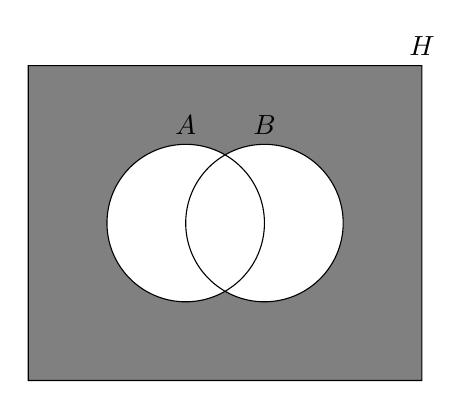
\begin{tikzpicture}[fill=gray]
% shade everything first
\fill (-2,-2) rectangle (3,2);

% then "erase" A
\fill[white] (0,0) circle (1);

% then "erase" B
\fill[white] (1,0) circle (1);

% outlines
\draw (0,0) circle (1) (0,1)  node [text=black,above] {$A$}
      (1,0) circle (1) (1,1)  node [text=black,above] {$B$}
      (-2,-2) rectangle (3,2) node [text=black,above] {$H$};
\end{tikzpicture}

So for every $x$ membership matches, hence the sets are equal.
\subsection*{2. \(\overline{A\cap B} = \overline{A}\cup\overline{B}\)}

Proof (element wise):
\[
\begin{aligned}
\forall x\!: \; x\in \overline{A\cap B}
&\iff x\notin (A\cap B)\\
&\iff \neg\big(x\in A \;\land\; x\in B\big)\\
&\iff \big(\neg(x\in A)\big)\lor\big(\neg(x\in B)\big)\\
&\iff (x\in\overline{A})\lor(x\in\overline{B})\\
&\iff x\in (\overline{A}\cup\overline{B}).
\end{aligned}
\]
So they match for every $x$, hence equal.

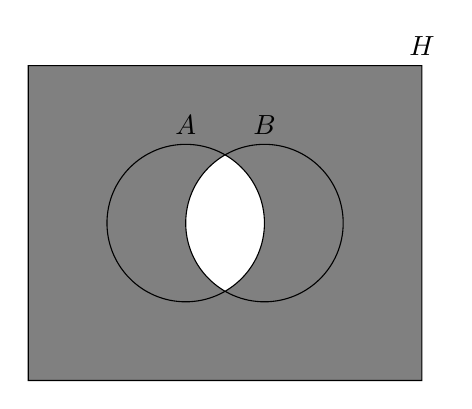
\begin{tikzpicture}[fill=gray]
% shade everything first
\fill (-2,-2) rectangle (3,2);

% then "erase" the intersection part (make it white)
\begin{scope}
  \clip (0,0) circle (1);
  \clip (1,0) circle (1);
  \fill[white] (-2,-2) rectangle (3,2);
\end{scope}

% outlines
\draw (0,0) circle (1) (0,1)  node [text=black,above] {$A$}
      (1,0) circle (1) (1,1)  node [text=black,above] {$B$}
      (-2,-2) rectangle (3,2) node [text=black,above] {$H$};
\end{tikzpicture}

\end{document}

